\documentclass{article}
\usepackage[paperwidth = 7.3cm, 
            paperheight = 6.9cm, 
            textwidth = 7.3cm,
            textheight = 6.9cm,
            centering]{geometry}
\usepackage{pgfplotstable}
\usepackage{amsmath,bm}
\usepackage{tikz}
\usetikzlibrary{arrows,
	arrows.meta,
	decorations.pathmorphing,
	calc,%
	decorations.pathmorphing,%
	decorations.markings,
	fadings,%
	shadings,%
	positioning,
	spy,
	shapes,
	shapes.geometric,
	shapes.arrows,
	fit,	plotmarks,}
\usepackage{tikz-dimline}

\pgfplotsset{
	width=5cm,
	height=2.5cm,
	scale only axis,
    %xmin   = 295,   xmax=330.72,
	%yticklabel style={/pgf/number format/fixed}, 
	every axis/.append style = {
		line width = 0.4pt,
		tick style = {line width=0.4pt,black},
		%tick label style={font=\tiny},
		every tick label/.append style={scale=0.75},
		major tick length = 0.8mm,
		minor tick length = 0.4mm,
		%axis line style = thick,
	},
	every axis plot/.append style={line width = 0.7pt,}
}
%\pgfplotsset{
%	compat=newest,
%	/pgfplots/legend image code/.code={%
%		\draw[mark repeat=1,mark phase=1,#1] 
%		plot coordinates {
%			(0cm,0cm) 
%			(0.0cm,0cm)
%			(0.0cm,0cm)
%			(0.0cm,0cm)
%			(0.3cm,0cm)%
%		};
%	},
%}
\pgfplotsset{
	compat=newest,
	/pgfplots/legend image code/.code={%
		\fill[#1,draw =none] (0cm,0.1cm) rectangle (0.2cm,-0.1cm);
	},
}
\def\eu{1.5327}
\def\ed{1.5412}
\def\hhu{-0.0047}
\def\hhd{-0.0055}
\def\lhu{-0.0097}
\def\lhd{-0.0164}




% \newlength{\bottomMargin}
% \setlength{\bottomMargin}{1mm}
% \setlength{\paperwidth}{7cm}
% \setlength{\paperheight}{10cm}
% \setlength{\pdfpagewidth}{\paperwidth}
% \setlength{\pdfpageheight}{\paperheight}
% \setlength{\textwidth}{\paperwidth}

\begin{document}
\thispagestyle{empty}
    \begin{tikzpicture}[overlay,remember picture,]
\node[anchor=north west,inner sep=0mm] at (current page.north west){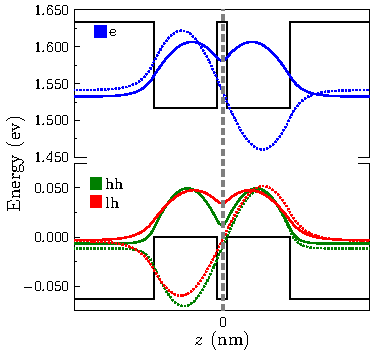
\includegraphics[width=0.49\linewidth]{out/numerical-results-m43523}};
\node[anchor=north east,inner sep=0mm] at (current page.north east){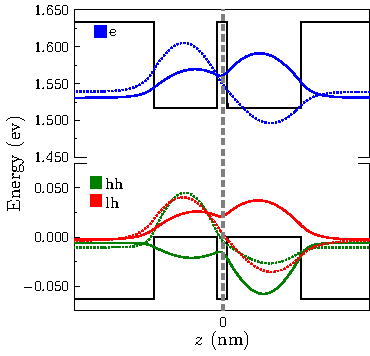
\includegraphics[width=0.49\linewidth]{out/numerical-results-m43522}};
\node[anchor=south west,inner sep=0mm] at (current page.south west){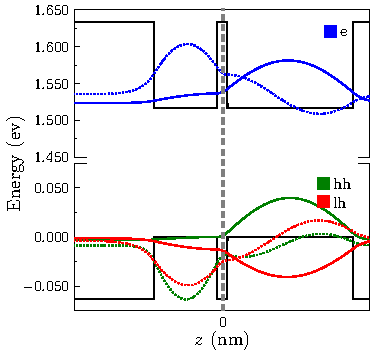
\includegraphics[width=0.49\linewidth]{out/numerical-results-m43521}};
\node[anchor=south east,inner sep=0mm] at (current page.south east){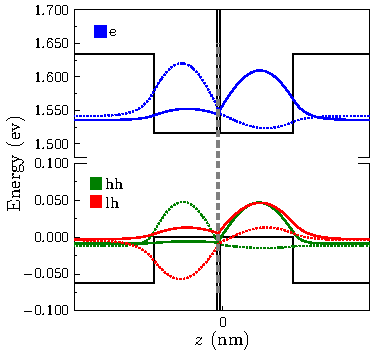
\includegraphics[width=0.49\linewidth]{out/numerical-results-m43172}};


\end{tikzpicture}
\end{document}